% Historical material for author review; submit separately only if the venue permits.
\documentclass[conference]{IEEEtran}
\usepackage{graphicx,booktabs,amsmath}
\begin{document}
\title{Supplementary Material: Historical Dengue Forecasting Analyses}
\author{\IEEEauthorblockN{University of Moratuwa research team}}
\maketitle

\section{Scope}
These materials preserve historical analyses omitted from the six-page manuscript.
They are development or legacy evidence, not results of the pending corrected-data or untouched-period evaluation.
The supplementary file is provided for author review; its eligibility for submission requires a venue decision.

\section{Source-series comparison}
\begin{figure}[h]
\centering
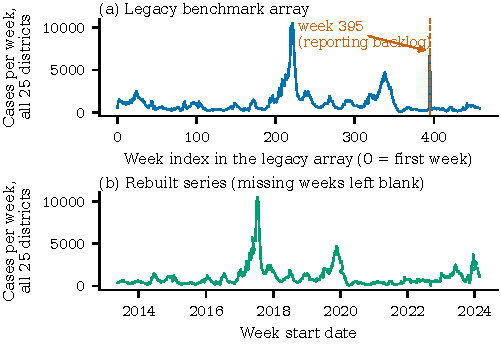
\includegraphics[width=\columnwidth]{figures/fig_data.pdf}
\caption{National weekly dengue notifications, summed over districts. (a) Legacy benchmark array; the dashed line marks the source-table formula error. (b) Rebuilt case series displayed on the repaired report calendar; missing reports interrupt the line. Repairing plot dates does not imply that historical model scores were rerun.}
\label{fig:data}
\end{figure}

\section{Legacy interval comparison}
The Gaussian-head results exist only on legacy-array folds containing the source-table error.
The persistence interval uses per-horizon training-residual quantiles; the scaled version divides residuals by the square root of one plus the latest count, then reverses that scaling for prediction.
Lower bounds are clipped at zero.
Coverage and width are averaged across folds, and no new model is trained for this comparison.
These historical intervals are not a calibration contribution of the rebuilt-data architecture.
\begin{table}[t]
\centering
\caption{Nominal 95\% intervals on the legacy-array folds (three folds, 68 test windows each). Coverage is the share of district-week targets inside the interval; width is the mean upper minus lower bound in cases. The first two rows need no network.}
\label{tab:interval}
\footnotesize
\begin{tabular}{@{}lrr@{}}
\toprule
Interval & Coverage (\%) & Width \\
\midrule
Persistence $\pm$ residual quantiles & 96.0 & 99 \\ % EV-142
Persistence $\pm$ scaled residual quantiles & 96.3 & 74 \\ % EV-143
\midrule
STGAT, Gaussian head & 95.6 & 123 \\ % EV-144
A3TGCN, Gaussian head & 96.2 & 230 \\ % EV-145
ASTGCN, Gaussian head & 94.7 & 128 \\ % EV-146
DCRNN, Gaussian head & 95.2 & 250 \\ % EV-147
AAGCN, Gaussian head & 95.9 & 145 \\ % EV-148
\bottomrule
\end{tabular}
\end{table}


\section{Stored development protocols}
\begin{table}[t]
\centering
\caption{Evaluation protocols, 3 seeds each. Persistence test RMSE (cases per district-week) differs between protocols because the test weeks differ, so numbers from different rows are never compared. Legacy array: with / without the backlog week.}
\label{tab:protocols}
\footnotesize
\setlength{\tabcolsep}{3pt}
\begin{tabular}{@{}lccr@{}}
\toprule
Protocol & Origins & Test share & Persistence \\
\midrule
Nine origins (main) & 0.50 to 0.90 by 0.05 & 5\% & 28.54 \\ % EV-141
Three origins & 0.55, 0.70, 0.85 & 15\% & 36.02 \\ % EV-141
Legacy array & 0.55, 0.70, 0.85 & 15\% & 44.80 / 29.52 \\ % EV-141
\bottomrule
\end{tabular}
\end{table}

\section{Historical three-origin ablations}
Table~\ref{tab:p3} shows the three-origin ablation, which we read as indicative only.
With three origins no gap can reach $p$ below 0.25. % EV-181
The simple graph control, a GCN with a residual head, scores 34.50 against 36.02 for persistence. % EV-116, EV-115
Removing the graph gives 34.57 and a learned adjacency gives 34.17, so the whole spread across the three graph choices is 0.41 cases, well inside the standard deviation of 10 to 11 over runs. % EV-117, EV-118, EV-116, EV-187
Under the shared fixed training settings, direct heads have high error on two adapted encoders: STGAT scores 62.00 and DCRNN scores 73.52 against persistence at 36.02. % EV-123, EV-125, EV-115
Their gated SEIR versions score 35.84 and 35.52. % EV-124, EV-126

\begin{table*}[t]
\centering
\caption{Indicative ablation on the three-origin protocol (rebuilt data, origins 0.55, 0.70, 0.85, 3 seeds, 9 runs per row). With three origins an exact sign-flip test cannot return $p<0.25$, so none of these gaps is tested. RMSE in cases per district-week; $\pm$ is the standard deviation over the nine runs. $\Delta$ is test RMSE minus the GCN control (graph layer, residual head), averaged over the nine matched runs; Wins counts runs out of nine. Do not compare these numbers with Table~\ref{tab:main}: the test weeks differ.}
\label{tab:p3}
\footnotesize
\setlength{\tabcolsep}{4pt}
\begin{tabular}{@{}lrrrrrrr@{}}
\toprule
Model & Val & $h{=}1$ & $h{=}2$ & $h{=}3$ & Test RMSE & $\Delta$ & Wins \\
\midrule
Persistence (last week) & 17.86 & 29.62 & 35.13 & 42.11 & 36.02 $\pm$ 12.41 & -- & -- \\ % EV-115 (EV-020)
\midrule
GCN, residual (graph control) & 16.84 & 28.28 & 34.01 & 40.13 & 34.50 $\pm$ 10.41 & -- & -- \\ % EV-116
No graph, residual & 16.90 & 28.54 & 34.05 & 40.08 & 34.57 $\pm$ 11.09 & +0.07 & 6/9 \\ % EV-117
Adaptive GCN (simple), residual & 16.69 & 28.44 & 33.97 & 39.20 & 34.17 $\pm$ 10.72 & $-$0.33 & 7/9 \\ % EV-118
\midrule
AAGCN, direct & 16.71 & 29.34 & 34.79 & 40.36 & 35.15 $\pm$ 11.53 & +0.65 & 4/9 \\ % EV-119
AAGCN, gated & 16.57 & 27.78 & 32.89 & 38.93 & 33.53 $\pm$ 10.14 & $-$0.97 & 9/9 \\ % EV-120
AAGCN, SEIR, free rate & 24.01 & 35.04 & 50.29 & 59.92 & 49.54 $\pm$ 18.49 & +15.04 & 0/9 \\ % EV-121
AAGCN, gated SEIR, free rate & 17.43 & 28.68 & 35.33 & 41.46 & 35.58 $\pm$ 11.50 & +1.08 & 3/9 \\ % EV-122
STGAT, direct & 22.93 & 60.24 & 61.97 & 63.67 & 62.00 $\pm$ 25.54 & +27.50 & 0/9 \\ % EV-123
STGAT, gated SEIR, free rate & 17.63 & 28.34 & 35.30 & 42.39 & 35.84 $\pm$ 11.65 & +1.34 & 3/9 \\ % EV-124
DCRNN, direct & 34.64 & 73.19 & 73.53 & 73.84 & 73.52 $\pm$ 32.90 & +39.02 & 0/9 \\ % EV-125
DCRNN, gated SEIR, free rate & 17.67 & 28.34 & 34.94 & 41.88 & 35.52 $\pm$ 11.42 & +1.02 & 3/9 \\ % EV-126
AAGCN, direct, NB + season (B) & 15.51 & 32.17 & 37.91 & 41.79 & 37.54 $\pm$ 13.90 & +3.04 & 3/9 \\ % EV-127
AAGCN, direct, squared error + season & 16.27 & 30.52 & 35.57 & 40.90 & 35.94 $\pm$ 12.14 & +1.43 & 3/9 \\ % EV-128
\bottomrule
\end{tabular}
\end{table*}


To separate the anchor from the physics, we ran a gated head without the simulator.
On validation, the simulator has mixed effects for the three poorly fitted direct-head models: the SEIR head minus the gated head is $+0.66$ (STGAT), $0.00$ (A3T-GCN) and $-0.68$ (DCRNN) in RMSE. % EV-159, EV-160, EV-161
The anchor and gate account for 1.12, 1.00 and 0.96 of the repair. % EV-159, EV-160, EV-161
On test, the SEIR head is lower than the gated head by 0.62, 1.66 and 3.50. % EV-159, EV-160, EV-161
Validation and test disagree.
These mixed results do not isolate an accuracy gain from the simulator.
Equal validation-only tuning and matched adaptive-encoder controls are missing.

The best three-origin arm is AAGCN with a gated head, at 33.53 against 36.02 for persistence. % EV-120, EV-115
This gap is untested.
The nine-origin protocol contains no gated head without physics, and its ASTGCN arm with a residual head is 0.11 above persistence. % EV-107


\section{Seed variation and normalized skill}
Table~\ref{tab:seed} separates initialization variation from the between-origin variation underlying the paired intervals in the manuscript.
The complete CSV summary records all thirty stored non-persistence arms, including MAE, skill, paired intervals and mean within-origin seed standard deviation.
The displayed subset follows the main manuscript; no claim of significance is inferred from a positive skill.
\begin{table}[!ht]\centering
\caption{Additional descriptive statistics for the historical development comparison. Skill is the mean over origins of one minus model RMSE divided by persistence RMSE. Seed SD is the mean within-origin standard deviation over neural seeds; persistence is deterministic. Neither statistic is a significance test.}
\label{tab:seed}\small
\begin{tabular}{@{}p{1.8in}rr@{}}\toprule
Model & Skill & Seed SD \\\midrule
Persistence (last week) & +0.000 & 0.000 \\ % EV-200
GCN, direct & +0.019 & 0.617 \\ % EV-201
GCN, residual (baseline GNN) & +0.019 & 0.507 \\ % EV-202
LSTM, direct & +0.014 & 0.412 \\ % EV-203
ASTGCN, direct & -0.012 & 0.912 \\ % EV-204
AAGCN, direct & -0.007 & 1.429 \\ % EV-205
STGAT, direct & -0.600 & 4.733 \\ % EV-206
ASTGCN, residual & +0.009 & 0.536 \\ % EV-207
Adaptive GCN, residual & +0.028 & 0.743 \\ % EV-208
GCN, SEIR, free rate & -0.404 & 0.171 \\ % EV-209
GCN, gated SEIR, free rate & +0.008 & 0.190 \\ % EV-210
Adaptive GCN, SEIR, anchored & -0.027 & 0.843 \\ % EV-211
Adaptive GCN, gated SEIR, mass-action & +0.008 & 0.098 \\ % EV-212
GCN, gated SEIR, anchored & +0.033 & 0.292 \\ % EV-213
Adaptive GCN, gated SEIR, anchored & +0.040 & 0.419 \\ % EV-214
Adaptive GCN, gated SEIR, anchored, learned $E_0$ & +0.035 & 0.448 \\ % EV-215
\bottomrule\end{tabular}\end{table}

\end{document}
